% CS631 Advanced Programming in the UNIX Environment
% Author: Jan Schaumann <jschauma@netmeister.org>
% $Id: slides.tex,v 1.1 2005/11/20 18:42:12 jschauma Exp $

\documentclass[xga]{xdvislides}
\usepackage[landscape]{geometry}
\usepackage{graphics}
\usepackage{graphicx}
\usepackage{colordvi}

\begin{document}
\setfontphv

%%% Headers and footers
\lhead{\slidetitle}
\chead{CS631 - Advanced Programming in the UNIX Environment}
\rhead{Slide \thepage}
\lfoot{\Gray{Lecture 13: Encryption in a Nutshell, Defensive Coding}}
\cfoot{\relax}
\rfoot{\Gray{\today}}

\vspace*{\fill}
\begin{center}
	\Hugesize
		CS631 - Advanced Programming in the UNIX Environment\\
		-- \\
		(Only the most basic) Encryption in a Nutshell \\
		Defensive Coding
	\hspace*{5mm}\blueline\\ [1em]
	\Normalsize
		Department of Computer Science\\
		Stevens Institute of Technology\\
		Jan Schaumann\\
		\verb+jschauma@stevens.edu+\\
		\verb+https://www.cs.stevens.edu/~jschauma/631/+
\end{center}
\vspace*{\fill}

\subsection{Cryptography}
Cryptography can provide ``security'' in the areas of:
\begin{itemize}
	\item Authenticity
		\begin{itemize}
			\item {\em Is the party I'm talking to actually who I {\em think} it is?}
		\end{itemize}
	\item Accuracy or Integrity
		\begin{itemize}
			\item {\em Is the message I received in fact what was sent?}
		\end{itemize}
	\item Secrecy or Confidentiality
		\begin{itemize}
			\item {\em Did/could anybody else see (parts of) the message?}
		\end{itemize}
\end{itemize}


\subsection{How does encryption work?}
{\em Secrecy}:  Make sure that the data can only be read by those intended.

\subsection{How does encryption work?}
{\em Secrecy}:  Make sure that the data can only be read by those intended.
\begin{itemize}
	\item Alice and Bob agree on a way to transform data
	\item transformed data is sent over insecure channel
	\item Alice and Bob are able to get data out of the transformation
\end{itemize}
\addvspace{.5in}
\begin{center}
	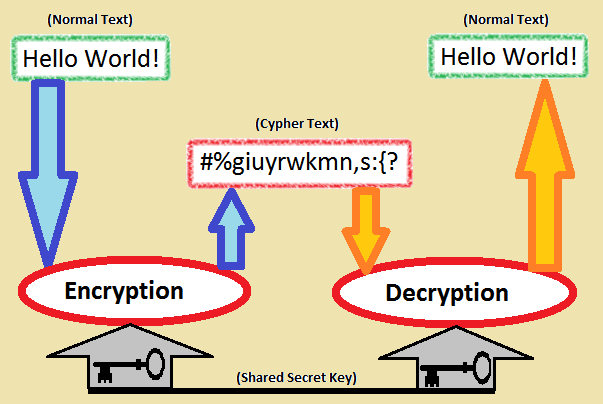
\includegraphics[scale=0.75]{pics/symmetric-key-crypto.eps}
\end{center}

\subsection{How does encryption work?}
Different approaches:
\begin{itemize}
	\item public key cryptography
	\item secret key cryptography
\end{itemize}

\subsection{How does encryption work?}
Different approaches:
\begin{itemize}
	\item public key cryptography (example: {\em RSA}, your ssh keys)
		\begin{itemize}
			\item Alice has a private and a public key
		\end{itemize}
\end{itemize}

\begin{center}
	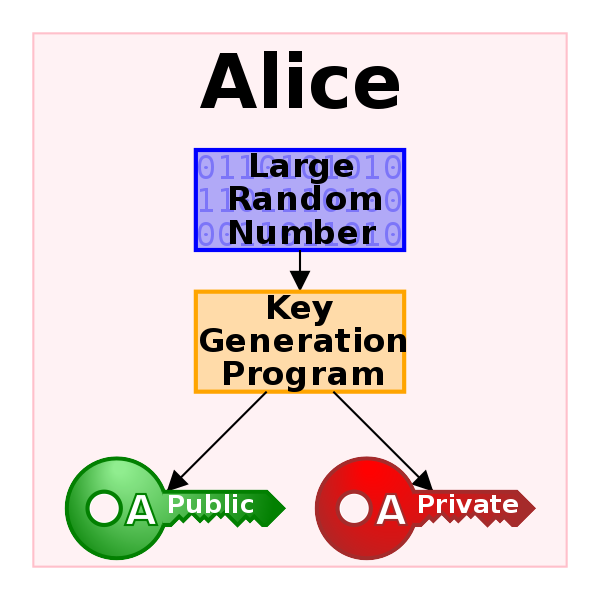
\includegraphics[scale=0.4]{pics/Public-key-crypto-1.eps}
 \end{center}


\subsection{How does encryption work?}
Different approaches:
\begin{itemize}
	\item public key cryptography (example: {\em RSA}, your ssh keys)
		\begin{itemize}
			\item Alice has a private and a public key
			\item data encrypted with her private key can only be decrypted by
				her public key and vice versa
		\end{itemize}
\end{itemize}

\begin{center}
	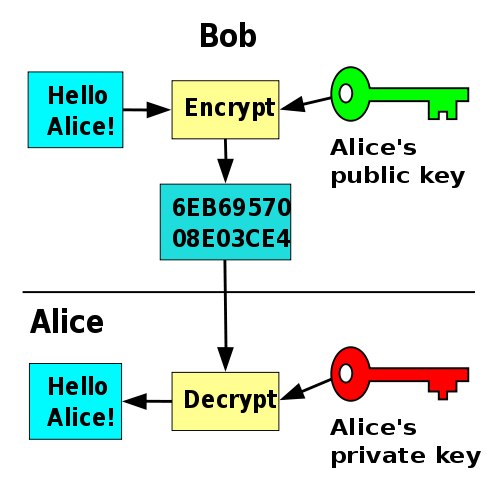
\includegraphics[scale=0.4]{pics/Public_key_encryption.eps}
 \end{center}


\subsection{How does encryption work?}
Different approaches:
\begin{itemize}
	\item public key cryptography (example: {\em RSA}, your ssh keys)
		\begin{itemize}
			\item Alice has a private and a public key
			\item data encrypted with her private key can only be decrypted by
				her public key and vice versa
			\item shared secrets derived from public key cryptography can be used as e.g. symmetric session keys
		\end{itemize}
\end{itemize}

\begin{center}
	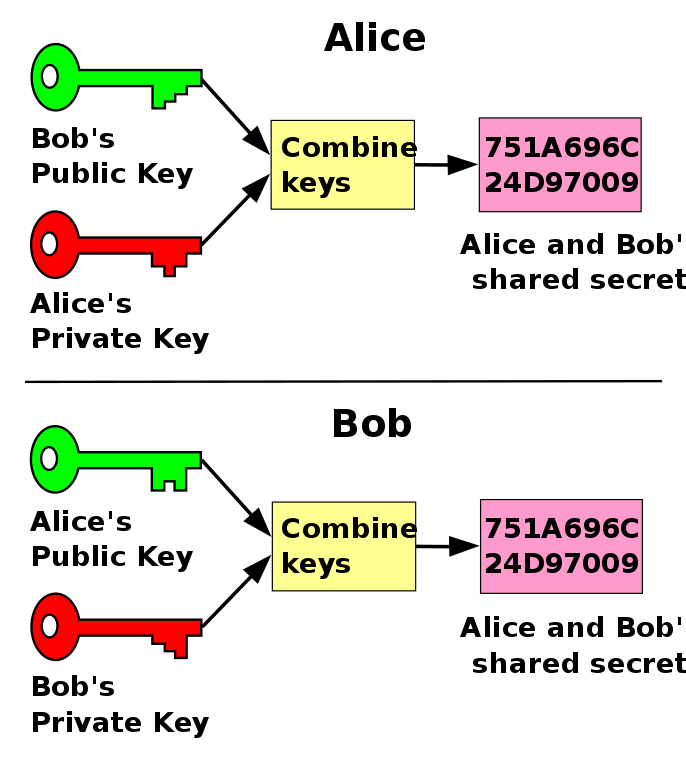
\includegraphics[scale=0.25]{pics/Public_key_shared_secret.eps}
 \end{center}

\subsection{How does encryption work?}
Different approaches:
\begin{itemize}
	\item secret key cryptography (example: {\em AES})
		\begin{itemize}
			\item Alice and Bob share a secret key
			\item for authentication purposes, Alice may prove
				to Bob that she knows the secret key
			\item any data encrypted with this key
				can also be decrypted using the same key
		\end{itemize}
\end{itemize}

 \begin{center}
        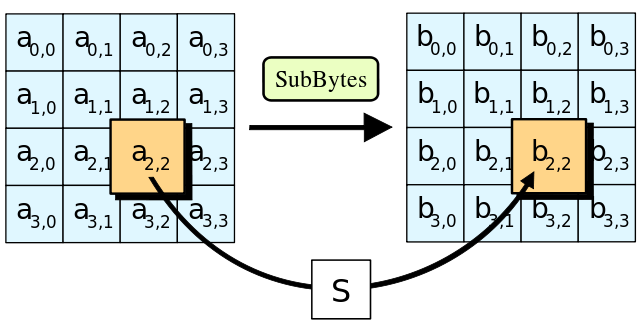
\includegraphics[scale=0.4]{pics/aes.eps}
 \end{center}

\subsection{Cipher Modes}
Encryption entails transformation of input data (``plain''
or ``clear'' text) into encrypted output data
(``ciphertext'').  Input data is generally transformed
in one of two ways:
\\

{\em Stream Cipher}: each bit of plaintext is combined
with a pseudo-random cipher digit stream (or {\em keystream})
\\

{\em Block Cipher}: fixed-length blocks of plaintext
are transformed into same-sized blocks of ciphertext;
may require padding


\subsection{Electronic Codebook Mode}
\begin{figure}[hb]
    \begin{center}
        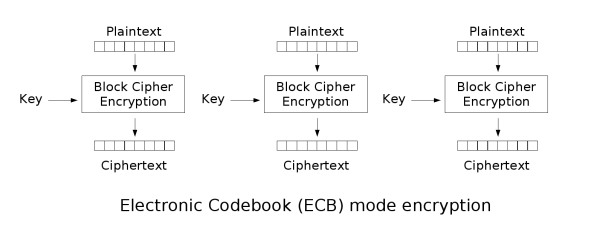
\includegraphics[scale=0.85]{pics/Ecb_encryption.eps} \\
        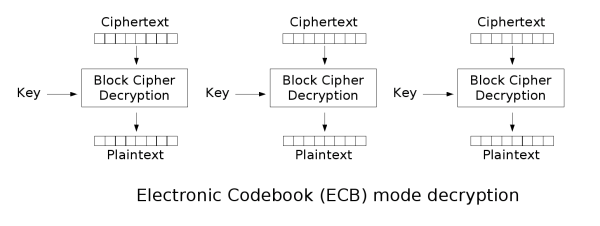
\includegraphics[scale=0.85]{pics/Ecb_decryption.eps} \\
    \end{center}
\end{figure}

\subsection{Electronic Codebook Mode}
\begin{center}
	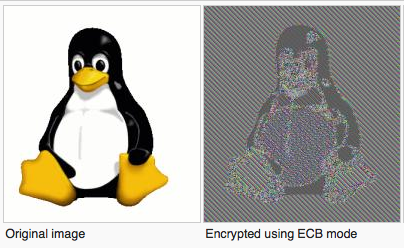
\includegraphics{pics/ecb.eps}
\end{center}


\subsection{Cipher Block Chaining}
\begin{figure}[hb]
    \begin{center}
        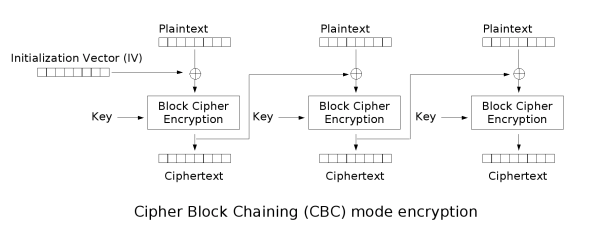
\includegraphics[scale=0.85]{pics/Cbc_encryption.eps} \\
        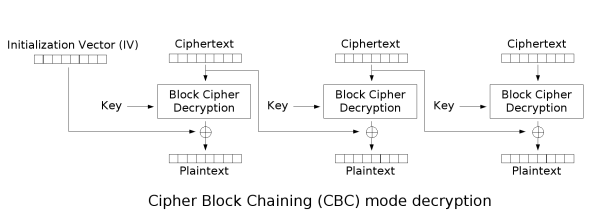
\includegraphics[scale=0.85]{pics/Cbc_decryption.eps}
    \end{center}
\end{figure}

\subsection{Using Crypto}

\begin{itemize}
	\item don't write your own crypto code, use existing libraries
	\item don't invent your own security protocol,
		even if you can't think of a way that you could break it
	\item don't invent your own source of entropy
	\item always seed your PRNG, salt your hashes
	\item default to reasonable crypto primitives:
		\begin{itemize}
			\item 2048 bit RSA for asymmetric key cryptography
			\item AES256-CBC for symmetric key cryptography
			\item HMAC-SHA256 for integrity
		\end{itemize}
\end{itemize}


\subsection{Random String generation}
Random numbers can be generated using {\tt /dev/random}, {\tt
/dev/urandom}, {\tt rand(3)}, {\tt random(3)}, {\tt BN\_rand(3)} etc.
\\

Map numbers to printable characters (for use as a salt, for example):

\begin{verbatim}
static const unsigned char itoa64[] =
        "./0123456789ABCDEFGHIJKLMNOPQRSTUVWXYZabcdefghijklmnopqrstuvwxyz";

char salt[16];
for (i=0; i<16; i++)
        salt[i] = itoa64[(int)random()%64];

\end{verbatim}
See also: \verb+rand.c+ from Lecture 11.

\subsection{On being random...}
\begin{center}
        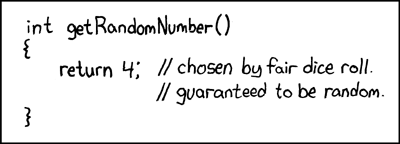
\includegraphics[scale=1]{pics/random_number.eps}
\end{center}

\subsection{On being random...}
\begin{center}
        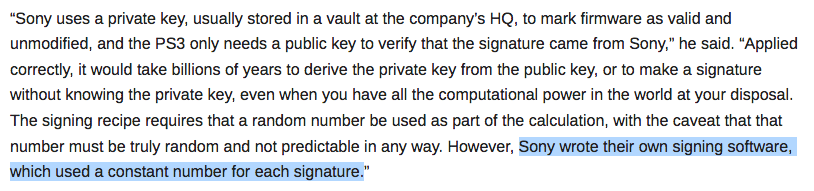
\includegraphics[scale=0.8]{pics/sony-ps3.eps}
\end{center}

\verb+https://youtu.be/LP1t_pzxKyE+ \\
\verb+https://is.gd/7Dmtwv+

\subsection{On being random...}

\begin{verbatim}
$ cc -Wall prng.c
$ ./a.out
      16807       692375228       699350133
$ ./a.out
      16807       692476070       699501396
$ ./a.out ; echo ; ./a.out
      16807       692593719       699652659

      16807       692593719       699669466
\end{verbatim}


\subsection{Handling Secrets}
{\bf Never} hardcode secrets in your code. \\

\begin{center}
        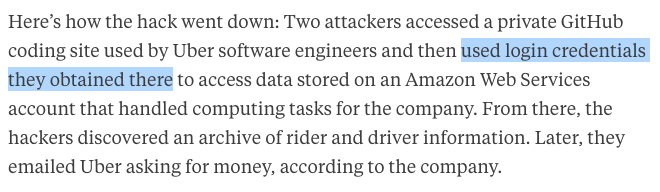
\includegraphics[scale=1]{pics/uber.eps}
\end{center}

\verb+https://is.gd/qRe7Z5+ \\
\verb+https://is.gd/ZaJDsT+

\subsection{Handling Secrets}
\begin{itemize}
	\item use a Key Management System; integrate
		with common libraries/API
	\item allow the user different options of
		prividing secrets; see e.g. \verb+openssl(1)+
		\begin{itemize}
			\item on the command-line (note:
			visible in process table!)
			\item via the environment (note:
			possibly visible to other users;
			often then stored in shell
			initialization files)
			\item from a file (note: ensure
			correct permissions!)
			\item from a file descriptor
			\item from stdin
			\item prompt from the tty
		\end{itemize}
	\item sanitize / zero out secrets after use
	\item don't log secrets!
\end{itemize}

\subsection{Handling Secrets}
\begin{verbatim}
$ cc -Wall getpass.c
$ echo foo | ./a.out
$ echo foo | env SECRET=password ./a.out
$ ./a.out -p password
^Z
$ ps wwaux | grep a.out
\end{verbatim}

\subsection{Input validation}

{\bf All data is tainted until proven otherwise.} \\

\begin{center}
        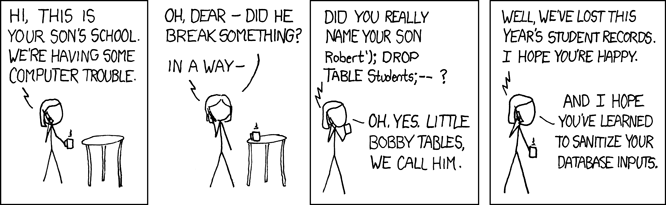
\includegraphics[scale=1]{pics/exploits_of_a_mom.eps}
\end{center}

\subsection{Input validation}

{\bf Never} trust anything from outside of your
control.  This includes:
\begin{itemize}
	\item data input directly provided by the user
	\item data indirectly / implicitly controlled
		by the user (e.g. HTTP headers)
	\item data read from files you think you
		control (e.g. config or state files)
	\item anything from the environment;
		\begin{itemize}
			\item use \verb+getpwent(3)+ instead of e.g. \verb+HOME+ or \verb+USER+
			\item explicitly set e.g. \verb+PATH+, \verb+LD_LIBRARY_PATH+
			\item explicitly unset e.g. \verb+LD_PRELOAD+
		\end{itemize}
\end{itemize}

\subsection{Input validation}
\begin{itemize}
	\item length checks (in both directions!)
	\item range checks on numeric fields, character ranges
	\item check path names against directory escapes (\verb+../../../+)
	\item prefer whitelists over blacklists
	\item encode data before validation or use
	\item use type check assertions
\end{itemize}

\subsection{Type Checks}
Prefer "is a" tests over "looks like": \\

\begin{tabular}{l l}
\begin{minipage}{4in}
\small
\begin{verbatim}
if (inet_pton(AF_INET, $ip)) {
        // AF_INET
} elsif (inet_pton(AF_INET6, $ip)) {
        // AF_INET6
} else {
        // not an IP address
}
\end{verbatim}
\Normalsize
\end{minipage} & \begin{minipage}{3in}
\small
IPv4:
\begin{verbatim}
(25[0-5]|2[0-4][0-9]|[01]?[0-9][0-9]?)\.(25[0-5]|2[0-4][0-9]|[01]?
[0-9][0-9]?)\.(25[0-5]|2[0-4][0-9]|[01]?\.(25[0-5]|2[0-4][0-9]|[01]
?[0-9][0-9]?)\.(25[0-5]|2[0-4][0-9]|[01]?[0-9][0-9]?)
\end{verbatim}

IPv6:
\begin{verbatim}
(([0-9a-fA-F]{1,4}:){7,7}[0-9a-fA-F]{1,4}|([0-9a-fA-F]{1,4}:){1,7}:|
([0-9a-fA-F]{1,4}:){1,6}:[0-9a-fA-F]{1,4}|([0-9a-fA-F]{1,4}:){1,5}(:
[0-9a-fA-F]{1,4}){1,2}|([0-9a-fA-F]{1,4}:){1,4}(:[0-9a-fA-F]{1,4}){1
,3}|([0-9a-fA-F]{1,4}:){1,3}(:[0-9a-fA-F]{1,4}){1,4}|([0-9a-fA-F]{1,
4}:){1,2}(:[0-9a-fA-F]{1,4}){1,5}|[0-9a-fA-F]{1,4}:((:[0-9a-fA-F]{1,
4}){1,6})|:((:[0-9a-fA-F]{1,4}){1,7}|:)|fe80:(:[0-9a-fA-F]{0,4}){0,4
}%[0-9a-zA-Z]{1,}|::(ffff(:0{1,4}){0,1}:){0,1}((25[0-5]|(2[0-4]|1{0,
1}[0-9]){0,1}[0-9])\.){3,3}(25[0-5]|(2[0-4]|1{0,1}[0-9]){0,1}[0-9])|
([0-9a-fA-F]{1,4}:){1,4}:((25[0-5]|(2[0-4]|1{0,1}[0-9]){0,1}[0-9])\.
){3,3}(25[0-5]|(2[0-4]|1{0,1}[0-9]){0,1}[0-9]))
\end{verbatim}
\Normalsize
\end{minipage}
\end{tabular}

\subsection{Subprocesses}
\begin{itemize}
	\item don't use \verb+system(3)+, \verb+popen(3)+ with any user provided input
	\item prefer \verb+fork(2)+/\verb+exec(3)+
	\item explicitly set a trusted \verb+PATH+, \verb+LD_*+ etc.
	\item never invoke commands from a temporary or relative location (e.g. \verb+/tmp/cmd+, \verb+./cmd+)
	\item set a suitable \verb+umask(2)+
\end{itemize}

\subsection{Setuid}
\begin{itemize}
	\item drop privileges as early as possible
	\item only raise privileges for sections you need
	\item permanently drop privileges if you no longer need them
	\item be aware of which subprocesses might let you break out of your program or which could spawn a shell (e.g. \verb+vi(1)+)
	\item be aware of which operations are atomic and which aren't
	\item beware signal and exit handlers
\end{itemize}

\subsection{File I/O}

\begin{itemize}
	\item avoid wherever possible
	\item assert suitable protection on private files (see e.g. \verb+ssh(1)+)
	\item be careful when opening, unlinking, overwriting files based on user input / user provided pathnames
	\item don't use temporary files
		\begin{itemize}
			\item set a restrictive \verb+umask(2)+
			\item use \verb+mktemp(3)+
			\item unlink via exit handler
		\end{itemize}
\end{itemize}

\verb+https://www.netmeister.org/blog/mktemp.html+

\subsection{Coding style}
Always use braces.
\begin{center}
        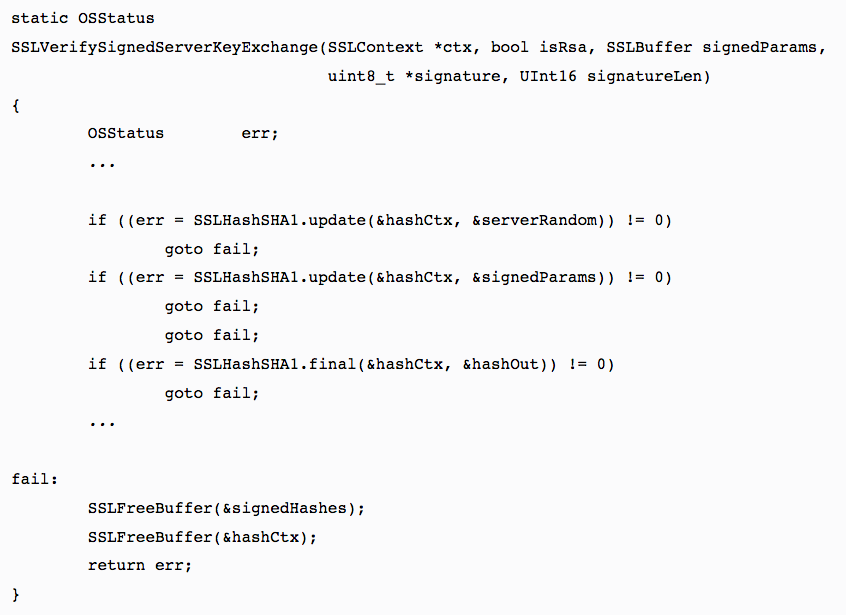
\includegraphics[scale=0.5]{pics/gotofail.eps}
\end{center}
\verb+https://www.imperialviolet.org/2014/02/22/applebug.html+

\subsection{Coding techniques}
\begin{itemize}
	\item treat functions as black boxes, minimize side-effects, avoid global variables
	\item explicitly mark variables / function arguments as '\verb+const+' (see also: \verb+const.c+)
	\item check your return codes!
	\item avoid magic numbers
	\item use \verb+strncpy(3)+/\verb+strncat(3)+ etc. instead of \verb+strcpy(3)+/\verb+strcat(3)+ etc.
	\item fail early, fail explicitly
	\item allocate / free resource in same scope
	\item check the boundaries of your buffers
	\item use compiler options (e.g. \verb+-fsanitize=address+), debugging libraries, analysis tools (e.g. valgrind)
	\item understand and resolve {\em all} compiler warnings (\verb+-Wall -Werror -Wpedantic+)
\end{itemize}

\subsection{Use-after-free}
\begin{center}
        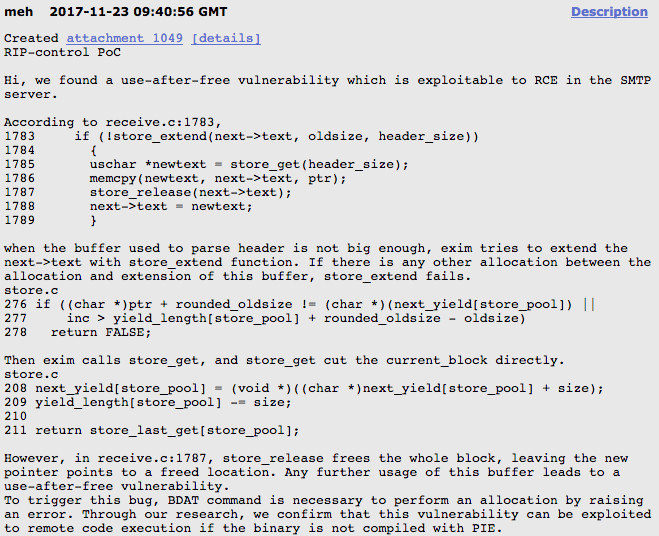
\includegraphics[scale=0.6]{pics/exim.eps} \\
	\verb+https://bugs.exim.org/show_bug.cgi?id=2199+
\end{center}

\subsection{Core Principles}

\begin{itemize}
	\item Simplify -- don't write any code you don't need.
	\item Minimize your Attack Surface -- only expose (interfaces, API functionality, access, ...) what is needed
	\item Secure Defaults -- user and group permissions,
		umask, PATH, locations, ...
	\item Assume that Human Behavior Will Introduce Vulnerabilities into Your System
	\item Know Your Enemy -- understand your threat model
\end{itemize}

\subsection{Core Principles}

\begin{itemize}
	\item Principle of Least Privilege -- only access, use, or accept
		information/resources that are strictly needed; don't run
		unprivileged unless/until privileged mode is needed
	\item Fail Closed -- (unexpected) failure must
		not lead to e.g. access, information disclosure,
		increased privileges, ...
	\item Defense in Depth -- any component or tool needs to be safe
		to use; do not rely on outside mechanisms or protections
	\item Kerkhoff's Principle -- "the enemy knows the system"; avoid Security by Obscurity
	\item Assume a Hostile Environment
		\begin{itemize}
			\item always use transport encryption
			\item always authenticate all parties
			\item authentication $!=$ authorization
		\end{itemize}
\end{itemize}
%
% \subsection{Practical AES}
% \begin{itemize}
%	\item a symmetric block cipher
%	\item variable key length
%	\item consists of a key setup phase and the actual encryption or
%		decryption
%	\item keying material use of {\tt ivec}, which needs to be shared
%	\item useful code examples in {\tt EVP\_EncryptInit(3)}
% \end{itemize}
%
%
% \subsection{HW\#4}
% \begin{verbatim}
% https://www.cs.stevens.edu/~jschauma/631/f15-hw4.html
% \end{verbatim}
% \begin{verbatim}
%
% NAME
%      aed - perform aes256‐cbc encryption/decryption
%
% DETAILS
%      aed reads data from stdin and either encrypts or decrypts it (depending
%      on the -d or -e flag).  It uses AES 256bit CBC mode with a SHA1 digest
%      with keying material derived from the passphrase using the
%      EVP_BytesToKey(3) function, generating a suitable salt via RAND_bytes(3).
%
%      Output is written to stdout.
%
%      When encrypting, the output is prefixed by the string "Salted__",
%      followed by the 8 byte salt.
% \end{verbatim}
% \Normalsize
%
% \subsection{HW\#4}
% \begin{verbatim}
% https://www.cs.stevens.edu/~jschauma/631/f15-hw4.html
% \end{verbatim}
% \begin{verbatim}
%
%      To encrypt the contents of the file ’file’ and storing the encrypted out-
%      put in ’file.enc’:
%
%            aed -e -p passfile <file >file.enc
%
%      To decrypt the contents of that file again:
%
%            aed -d -p passfile <file.enc
%
%      Since aed operates on stdin and stdout, the above two commands could also
%      be chained:
%
%            export AED_PASS=$(cat passfile)
%            cat file | aed -e | aed -d
% \end{verbatim}
% \Normalsize
%
\subsection{References and Links}
Crypto:
\begin{itemize}
	\item {\tt crypto(3)}
	\item {\tt EVP\_EncryptInit(3)}
	\item {\tt EVP\_BytesToKey(3)}
	\item {\tt http://tldp.org/LDP/LG/issue87/vinayak.html}
	\item {\tt http://en.wikipedia.org/wiki/Cipher\_Block\_Chaining}
	\item {\tt https://is.gd/khpsCT}
\end{itemize}

\subsection{References and Links}
Defensive Coding
\begin{itemize}
	\item \verb+https://is.gd/ChD04C+
	\item \verb+https://is.gd/ee4nXr+
	\item \verb+https://www.owasp.org/index.php/Data_Validation+
	\item \verb+https://www.netmeister.org/blog/mktemp.html+
	\item \verb+https://is.gd/JVS5lI+
	\item \verb+http://valgrind.org/docs/manual/mc-manual.html+
	\item \verb+https://is.gd/QMru7v+
	\item \verb+https://www.netmeister.org/blog/threat-model-101.html+
\end{itemize}

\subsection{References and Links}
Bugs and exploits
\begin{itemize}
	\item \verb+http://enderunix.org/docs/en/bof-eng.txt+
	\item \verb+https://bugs.exim.org/show_bug.cgi?id=2199+
	\item \verb+https://is.gd/7Dmtwv+
	\item \verb+https://is.gd/qRe7Z5+
	\item \verb+https://is.gd/ZaJDsT+
	\item \verb+https://www.imperialviolet.org/2014/02/22/applebug.html+
\end{itemize}


\end{document}
